
\documentclass[nooutcomes]{ximera}
%\documentclass[space,handout,nooutcomes]{ximera}

% For preamble materials

\usepackage{pgf,tikz}
\usepackage{mathrsfs}
\usetikzlibrary{arrows}
\usepackage{framed}
\usepackage{amsmath}
%\pgfplotsset{compat=1.16}

\graphicspath{
  {./}
  {algorithms/}
  {../algorithms/}
}

\pdfOnly{\renewenvironment{image}[1][]{\begin{center}}{\end{center}}}

%%% This set of code is all of our user defined commands
\newcommand{\bysame}{\mbox{\rule{3em}{.4pt}}\,}
\newcommand{\N}{\mathbb N}
\newcommand{\C}{\mathbb C}
\newcommand{\W}{\mathbb W}
\newcommand{\Z}{\mathbb Z}
\newcommand{\Q}{\mathbb Q}
\newcommand{\R}{\mathbb R}
\newcommand{\A}{\mathbb A}
\newcommand{\D}{\mathcal D}
\newcommand{\F}{\mathcal F}
\newcommand{\ph}{\varphi}
\newcommand{\ep}{\varepsilon}
\newcommand{\aph}{\alpha}
\newcommand{\QM}{\begin{center}{\huge\textbf{?}}\end{center}}

\renewcommand{\le}{\leqslant}
\renewcommand{\ge}{\geqslant}
\renewcommand{\a}{\wedge}
\renewcommand{\v}{\vee}
\renewcommand{\l}{\ell}
\newcommand{\mat}{\mathsf}
\renewcommand{\vec}{\mathbf}
\renewcommand{\subset}{\subseteq}
\renewcommand{\supset}{\supseteq}
\renewcommand{\emptyset}{\varnothing}
\newcommand{\xto}{\xrightarrow}
\renewcommand{\qedsymbol}{$\blacksquare$}
\newcommand{\bibname}{References and Further Reading}
\renewcommand{\bar}{\protect\overline}
\renewcommand{\hat}{\protect\widehat}
\renewcommand{\tilde}{\widetilde}
\newcommand{\tri}{\triangle}
\newcommand{\minipad}{\vspace{1ex}}
\newcommand{\leftexp}[2]{{\vphantom{#2}}^{#1}{#2}}

%% More user defined commands
\renewcommand{\epsilon}{\varepsilon}
\renewcommand{\theta}{\vartheta} %% only for kmath
\renewcommand{\l}{\ell}
\renewcommand{\d}{\, d}
\newcommand{\ddx}{\frac{d}{dx}}
\newcommand{\dydx}{\frac{dy}{dx}}


\usepackage{bigstrut}


\newenvironment{sectionOutcomes}{}{}

\usepackage{array}
%\setlength{\extrarowheight}{-.2cm}   % Commented out by Findell to fix table headings.  Was this for typesetting division?  
\newdimen\digitwidth
\settowidth\digitwidth{9}
\def~{\hspace{\digitwidth}}
\def\divrule#1#2{
\noalign{\moveright#1\digitwidth
\vbox{\hrule width#2\digitwidth}}}


\title{Polynomials}
\author{Bart Snapp and Brad Findell}
\begin{document}
\begin{abstract}
Problems about polynomials 
\end{abstract}
\maketitle

\begin{problem}Explain what is meant by a \textit{polynomial} in a variable $x$.
\end{problem} 

\begin{problem}Given:
\[
3x^7 -x^5 + x^4 -16x^3 + 27 = a_7 x^7 + a_6x^6 + a_5x^5 + a_4x^4 + a_3x^3 + a_2x^2 + a_1x^1 + a_0
\]
Find $a_0$, $a_1$, $a_2$, $a_3$, $a_4$, $a_5$, $a_6$, $a_7$.
\end{problem} 

\begin{problem}Given:
\[
6x^5+a_4 x^4 -x^2 + a_0 = a_5 x^5 - 24 x^4 + a_3 x^3 + a_2 x^2 - 5
\]
Find $a_0$, $a_1$, $a_2$, $a_3$, $a_4$, $a_5$.
\end{problem} 

\begin{problem}Is it true that polynomials are equal if and only if their
  coefficients are equal? Explain your reasoning.
\end{problem} 

\begin{problem}Is it true that numbers are equal if and only if their digits
  are equal? Explain your reasoning.
\end{problem} 

\begin{problem}Explain how to add two polynomials.  Explain, in particular, how ``collecting like terms'' is
an application of the properties of arithmetic.  
\end{problem} 

\begin{problem}Explain how to multiply two polynomials.
\end{problem} 

\begin{problem}Here is an example of the polynomial division algorithm:
\begin{image}  
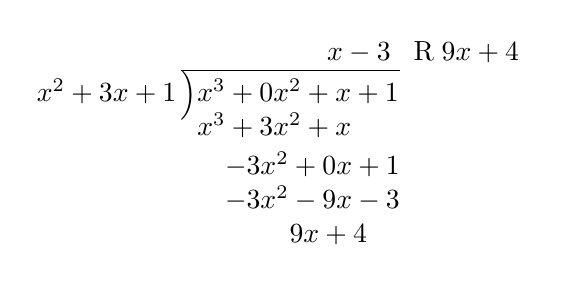
\begin{tikzpicture}  
\node at (0,0) {
$x^2 + 3x + 1\,\begin{tabular}[b]{@{}r@{}r} 
$x-3$~~&\, R\;$9x+4$\\ 
\cline{1-1}
\Big)\begin{tabular}[t]{@{}l@{}} \bigstrut[t] $x^3 + 0x^2 + x + 1$\\ 
$x^3 + 3x^2 + x$ \\ 
\divrule{0}{11}  
\bigstrut[t]~~~$-3x^2 +0x + 1$\\
~~~$-3x^2-9x -3$\\
\divrule{4}{12}
~~~~~~~~~~$9x + 4$
\end{tabular}
\end{tabular}$
};
\end{tikzpicture}
\end{image}

\begin{enumerate}
\item Describe how to perform this algorithm.
\item Provide an additional relevant and revealing example
  demonstrating that you understand the algorithm.
\item Show the ``behind-the-scenes'' algebra that is going on here.
\end{enumerate}\index{division algorithm!polynomial}
\end{problem} 

\begin{problem}State the \textit{Division Theorem} for polynomials. Give some
  relevant and revealing examples of this theorem in action.
\end{problem} 

\begin{problem}Given a polynomial
\[
p(x) = a_nx^n + a_{n-1}x^{n-1} + \dots + a_1 x+ a_0
\]
can you find two numbers $L$ and $U$ such that $L \le p(x) \le U$ for
all $x$? If so, explain why. If not, explain why not.
\end{problem} \begin{problem}Consider all polynomials of the form
\[
a_nx^n + a_{n-1}x^{n-1} + \dots + a_1 x+ a_0
\]
where the $a_i$'s are integers. If you substitute an integer for $x$
will you always get an integer out? Explain your reasoning.
\end{problem} \begin{problem}Consider the following polynomial:
\[
p(x) = \frac{x^2}{2}+\frac{x}{2}
\]
Will $p(x)$ always returns an integer when an integer is substituted
for $x$? Explain your reasoning.

\end{problem} 

\begin{problem}Fix some integer value for $x$ and consider all polynomials of
  the form
\[
a_nx^n + a_{n-1}x^{n-1} + \dots + a_1 x+ a_0
\]
Where the $a_i$'s are integers greater than or equal to $0$. Which
numbers can be represented by such polynomials? Explain your
reasoning.
\end{problem} 

\begin{problem}Find a polynomial 
\[
p(x) = a_nx^n + a_{n-1}x^{n-1} + \dots + a_1 x+ a_0
\]
such that $a_i$'s are integers greater than or equal to $0$ and less
than $2$ such that $p(2) = 35$. Discuss how your answer compares to
the representation of $35$ in base two. Explain your reasoning.
\end{problem} 

\begin{problem}Find a polynomial 
\[
p(x) = a_nx^n + a_{n-1}x^{n-1} + \dots + a_1 x+ a_0
\]
such that $a_i$'s are integers greater than or equal to $0$ and less
than $7$ such that $p(7) = 234$. Discuss how your answer compares to
the representation of $234$ in base seven. Explain your reasoning. 
\end{problem} 

\begin{problem}Find a polynomial 
\[
p(x) = a_nx^n + a_{n-1}x^{n-1} + \dots + a_1 x+ a_0
\]
such that $a_i$'s are integers greater than or equal to $0$ and less
than $10$ such that $p(10) = 18$. Discuss how your answer compares to
the representation of $18$ in base ten. Explain your reasoning.
\end{problem} 

\begin{problem}Find a polynomial 
\[
p(x) = a_nx^n + a_{n-1}x^{n-1} + \dots + a_1 x+ a_0
\]
such that $a_i$'s are integers greater than or equal to $0$ and less
than $15$ such that $p(15) = 201$. Discuss how your answer compares to
the representation of $201$ in base fifteen. Explain your reasoning.
\end{problem} 

\begin{problem}Fix some integer value for $x$ and consider all polynomials of the form
\[
a_nx^n + a_{n-1}x^{n-1} + \dots + a_1 x+ a_0
\]
Where the $a_i$'s are integers greater than or equal to $0$ and less
than $x$. Which numbers can be represented by such polynomials?
Explain your reasoning. Big hint: Base $x$.
\end{problem} 

\begin{problem}Fix some integer value for $x$ and consider all polynomials of
  the form
\[
a_nx^n + a_{n-1}x^{n-1} + \dots + a_1 x+ a_0
\]
Where the $a_i$'s are integers greater than or equal to $0$ and less
than $10$. Which numbers can be represented by such polynomials?
Explain your reasoning.
\end{problem} 

\begin{problem}Consider $x^2 + x + 1$. This can be thought of as a ``number'' in
  base $x$. Express this number in base $(x+1)$, that is, find $b_0$, $b_1$, $b_2$ such that 
\[
b_2(x+1)^2 +b_1(x+1) + b_0 = x^2 + x + 1.
\]
Explain your reasoning.
\end{problem} 

\begin{problem}Consider $x^2 + 2x + 3$. This can be thought of as a ``number'' in
  base $x$. Express this number in base $(x-1)$, that is, find $b_0$, $b_1$, $b_2$ such that 
\[
b_2(x-1)^2 +b_1(x-1) + b_0 = x^2 + 2x + 3.
\]
Explain your reasoning.
\end{problem} 

\begin{problem}Consider $x^3 + 2x + 1$. This can be thought of as a ``number'' in
  base $x$. Express this number in base $(x-1)$, that is, find $b_0$, $b_1$, $b_2,$ $b_3$ such that 
\[
b_3(x-1)^3 + b_2(x-1)^2 +b_1(x-1) + b_0 = x^3 + 2x + 1.
\]
Explain your reasoning.
\end{problem} 

\begin{problem}If the polynomial
\[
p(x) = a_nx^n + a_{n-1}x^{n-1} + \cdots + a_1x + a_0
\]
is thought of as a ``number'' in base $x$, describe two different ways
to find the base $(x-1)$ coefficients of $p(x)$.
\end{problem}


\end{document}